\chapter{Experimente und Ergebnisse}\label{experiment}

\section{Evaluation der Gesichtserkennung}\label{evalfa}
Die Genauuigkeit der Position der Landmarks, im Verhältnis zu der Gesamtheit aller verfügbaren Patient*innen, werden für die 9 Bilder jedes einzelnen Patienten, zu allererst die Ausrechnung dieser vollzogen. Festgestellt wurde, das die Seitenverhältnisse und Größe der einzelnen Bilder des Datensatzes für das verwendete Framework \glqq Face-Alignment\grqq{} von Adrian Bulat und Georgios Tzimiropoulos, eine zu hohe Auflösung aufweisen und so die Landmarks nicht korrekt positioniert sind (Tabelle \ref{cap:fa_factor}). Durch Reverse Engineerung des Sourcecodes wurde festgestellt, dass die verwendeten Bildmaterialen zum trainieren der Neuronalen-Netze des Frameworks, indirekt eine Standartauflösung von maximal 1920x1080px (HD) haben \cite{fa_framework}.


Die Lösung für das Problem ist eine geschickte Verkleinerung der Größenverhältnisse in Abhängigkeit der tatsächlichen Bildgröße $(a, b)$. Dabei ist $a$ die Pixelanzahl in horizontaler und $b$ in vertikaler Richtung. Die Größe der Bilder werden dazu in den Bereich für die optimale Ausführung zur Generierung der Landmarks verkleinert. Der Faktor $F_{ab}$ für die Änderung der Bildgröße lässt sich wiefolgt berechnen:

\begin{equation}
F(a, b) = \begin{cases*}
  \frac{\max(a, b)}{10^{3}} $+ 1$,  & wenn $\max(a, b) \mod 2$  \\
  \frac{\max(a, b)}{10^{3}},        & sonst
\end{cases*}
\end{equation}

Nachdem die Landmarks vom System ausgerechnet wurden, werden diese auf das Origialbild mit der vollen Größe angewendet. Dazu werden alle Punkte mit $F_{ab}$ multipliziert. Für die spätere Anwendung in den Neuronalen-Netzen und der Auschneidung der Regionen, werden so die hochauflösenden Bilder verwendet. Damit auch die Patienenbilder, deren Landmarks teilweise von der Ideallineie abweichen, verwendet werden können, muss beim Ausscheiden ein Offset hinzu gerechnet werden.




\begin{table}[!htb]\vspace{1ex}\centering
  \begin{tabular}{cc|ccc|}
  \cline{3-5}
  \multirow{2}{*}{}      &       & \multicolumn{3}{c|}{Plazierung der Landmarks}                                               \\ \cline{3-5}
                         &       & \multicolumn{1}{c|}{korrekt} & \multicolumn{1}{c|}{teilweise} & falsch \\ \hline
  \multicolumn{1}{c|}{\multirow{2}{*}{\begin{tabular}[c]{@{}c@{}}vor Anpassung\\ der Bildgröße\end{tabular}}}  & \# & \multicolumn{1}{c|}{0} & \multicolumn{1}{c|}{12} & 639 \\ \cline{2-5}
  \multicolumn{1}{c|}{} & in \% & \multicolumn{1}{c|}{0}       & \multicolumn{1}{c|}{1.84}                 & 98.16      \\ \hline
  \multicolumn{1}{c|}{\multirow{2}{*}{\begin{tabular}[c]{@{}c@{}}nach Anpassung\\ der Bildgröße\end{tabular}}} & \# & \multicolumn{1}{c|}{572} & \multicolumn{1}{c|}{78} & 1 \\ \cline{2-5}
  \multicolumn{1}{c|}{} & in \% & \multicolumn{1}{c|}{87.87}       & \multicolumn{1}{c|}{11.98}                 & 0.15      \\ \hline
  \end{tabular}
  \caption[Plazierung der Landmarks vor und nach der Anpassung der Bildgröße durch den Faktor]{Plazierung der Landmarks vor und nach der Anpassung der Bildgröße durch den Faktor $F_{ab}$ bezogen auf die 86 Patient*innen des Datensatzes und deren vorhandenen Bilder}\label{cap:fa_factor}
\vspace{2ex}\end{table}\label{table:fa_factor}


Auch die Rotation der Bilder kann Mithilfe der Landmarks heraufgefunden und falls nötig korrigiert werden. Dazu werden die absoluten Positionen von zwei Marker miteinander verglichen. Experimentel lässt sich der Rotationswinkel $R$ gegen den Uhrzeigersinn durch einfaches Ausprobieren mit den Punkt 0 (linkes Ohr) und 8 (Kinn) so definieren:

\begin{equation}
R[P(0), P(8)] = \begin{cases*}
  270^{\circ}, & wenn $P_{a}(0) < P_{a}(8) \land P_{b}(0) > P_{b}(8)$ \\
  180^{\circ}, & wenn $P_{a}(0) > P_{a}(8) \land P_{b}(0) > P_{b}(8)$ \\
  90^{\circ} , & wenn $P_{a}(0) > P_{a}(8) \land P_{b}(0) < P_{b}(8)$ \\
  0^{\circ} , & sonst
\end{cases*}
\end{equation}

\textbf{TODO graphisch darstellen anhand der Punkte}


\clearpage
\section{Hyperparameter}\label{hyper}
\textbf{TODO}

\subsection{Teilung in Training und Validation}\label{split}
\textbf{TODO}

\subsection{Augmentierung}\label{augmentation}
\textbf{TODO}

\subsection{? Lernrate Scheduler Optimizer, lossfn}\label{lrate}
\textbf{TODO}

\begin{equation}
 loss(y, class) = - y[class] + log( \sum_{j}^{} e^{x[j]} )
\end{equation}

\section{Nachweis der Funktionsweise von Oversampling}\label{oversampling}
\textbf{TODO}


\section{Sequentiell}\label{sequent}
\textbf{TODO}

\section{Early Fusion}\label{earlyfusion}
\textbf{TODO}

\section{Late Fusion}\label{latefusion}
\textbf{TODO}










\clearpage
\section{Fusionierung der Module}\label{fusion}

\subsection{Automaten}\label{automata}
Um anahnd der einzelnen Module nun den Grad ermitteln zu können, wird ein Automat durchlaufen. Dabei ist der Endzustand der aus den Einzelergebnissen resultierender Grad des House-Brackmann Skala. Das Eingabewort in den Automat sind die Ausgabe der Module. Dabei kann das Wort aus den Bestandteilen bestehen:

\begin{itemize}
\setlength\itemsep{-0.5em}
\item $s = y_{symmetrie}  \in  0, 1, 2 $
\item $e = y_{lidschluss} \in  0, 1 $
\item $m = y_{mund}       \in  0, 1, 2, 3 $
\item $f = y_{strin}      \in  0, 1, 2 $
\end{itemize}

Fix ist das Eingabewort \flqq sefm\frqq in den Automaten. Durch den Nichtdeterminismus wird  entscheiden, wenn keine Änderung des Zustandes mehr möglich ist. Der erste Eingabebuchstabe wird aus der Eingabe genommen (\flqq sefm\frqq $\rightarrow$ \flqq efm\frqq). Dieser Prozess wird solange wiederholt, bis das Eingabewort vollständig abgearbeitet ist. Zu Beachten sind dabei die Übergangsfunktionen zwischen zwei Zusänden. Jeder Buchsabe im Einabewort hat eine Gewichtung (Ergebnis der Funktion), die entscheidet, ob der Pfad passierbar ist (Abb. \ref{cap:automata}).

\vspace{0.5cm}

Der Nicht-Deterministischer endlicher Automat für die Bestimmung des Grades nach der Hosue-Brackmann Skala besteht aus dem Fünftupel $N = (Q, \Sigma, \delta, q_0, F)$:

\begin{itemize}
\item $Q=\{ q_I, q_{II}, q_{III}, q_{IV}, q_{V}, q_{VI} \}$  ist eine endliche Zustandsmenge, wobei der Index representativ der Grad ist, der ermittelt werden soll.
%\item $\Sigma={y_{symmetrie}, y_{lidschluss}, y_{mund}, y_{strin}}$ ist ein endliches Alphabet (in dem Fall speziell die Ausgabe der Funktionen)
\item $\Sigma=\{ s, e, m, f \}$ ist ein endliches Alphabet (speziell begrenzt auf die Module)
\item $\delta:Q \times \Sigma \rightarrow P(Q)$ Nicht-Deterministische Übergangsfunktion (siehe Tabelle \ref{cap:transition})
\item $q_0=q_I$ ist der Startzustand
\item $F \subset Q = Q$ Menge aller akzeptierten Endzustände
\end{itemize}


\begin{table}[!tb]\vspace{1ex}\centering
  %\resizebox{10cm}{!}{
  \begin{tabular*}{16cm}{c||c|c|c|c|}
  %\backslashbox{Room}{Date}
  \backslashbox{$Q$}{$\Sigma$} & $s$ & $e$ & $m$ & $f$
  \\\hline\hline
  $q_I$    & $q_{V}$, wenn $s\geqslant1$&$q_{IV}$, wenn $e\geqslant1$&$q_{II}$, wenn $m\geqslant1$&$q_{III}$, wenn $f\geqslant1$\\
  $q_{II}$ & $\varnothing $             &$\varnothing $              &$q_{IV}$, wenn $m\geqslant2$&$\varnothing $               \\
  $q_{III}$& $\varnothing $             &$\varnothing $              &$q_{IV}$, wenn $m=2$        &$q_{IV}$, wenn $f=2$         \\
  $q_{IV}$ & $\varnothing $             &$\varnothing $              &$q_{VI}$, wenn $m=3$        &$\varnothing $               \\
  $q_{V}$  & $q_{VI}$, wenn $s=2$       &$\varnothing $              &$q_{VI}$, wenn $m=3$        &$\varnothing $               \\
  $q_{VI}$ & $\varnothing $             &$\varnothing $              &$\varnothing $              &$\varnothing $
  \\\hline
  \end{tabular*}
%  }
  \caption[Übergangsfunktion $\delta$ des Automaten für die Bestimmung des Grades]{Übergangsfunktion $\delta$ des Automaten für die Bestimmung des Grades}\label{cap:transition}
\vspace{2ex}\end{table}\label{table:transition}

%\definecolor{mycolor}{RGB}{50,180,255}
\begin{figure}[!tb]
\begin{center}
\begin{tikzpicture}[->,>=stealth',shorten >=1pt,auto,node distance=2.5cm,semithick]
  \tikzstyle{every state}=[fill=cyan,draw=black,text=black]

  \node[initial,state] (A)                    {$q_{I}$};
  \node[state]         (B) [right of=A]       {$q_{II}$};
  \node[state]         (C) [right of=B]       {$q_{III}$};
  \node[state]         (D) [right of=C]       {$q_{IV}$};
  \node[state]         (E) [right of=D]       {$q_{V}$};
  \node[state]         (F) [right of=E]       {$q_{VI}$};

  \path (A) edge                 node {$m\geqslant1$} (B)
            edge [bend right=40] node {$f\geqslant1$} (C)
            edge [bend right=40] node {$e=1$}         (D)
            edge [bend right=40] node {$s\geqslant1$} (E)
            edge [bend right=40] node {$s\geqslant1$} (E)
        (B) edge [bend left=40]  node {$m\geqslant2$} (D)
        (C) edge                 node {$f=2$}         (D)
            edge [bend right=40] node {$m=2$}         (D)
        (D) edge [bend left=40]  node {$m=3$}         (F)
            edge [bend left=40]  node {$m=3$}         (F)
        (E) edge                 node {$s=2$}         (F)
            edge [bend right=40] node {$m=3$}         (F);

\end{tikzpicture}
\caption[Gewichteter Automat dargestellt als Graph]{Gewichteter Automat dargestellt als Graph}\label{cap:automata}
\end{center}
\end{figure}\label{fig:automata}



\subsection{Mittelwertbildung der Zeilensumme}\label{rowsum}
\textbf{TODO}

















\clearpage
\section{Laufzeitanalyse des Caches}\label{analyze}
Analysiert wurde die Laufzeiten des Systems bezogen auf 5 Epochs und einer Anzahl von 53 Datensätzen. Dabei wurde der LRU-Cache Stückweise um eins inkrementiert. Wenn der \ac{lru} größer als die Anzahl der Datensätze ist, wird die Laufzeit stabil um einen Fixwert gehalten. Erklärbar ist dies dadurch, da jedes Element des Datensatzes im \ac{lru} liegt und somit keine Rechenzeit für die Berechnung verschwendet wird. Auch signifikant Feststellbar ist der rapide Zuwachs an Zeiteinheiten, wenn die Größe des \ac{lru} abnimmt. Dabei ist der Zeitzuwachs nicht linear. Die Hitrate (Trefferrate für im Cache liegende Elemente) nimmt mit vermindeter Größe ab. Mehr Elemente müssen zuerst berechnet werden. Ab einen Punkt ist kein Zeitzuwachs mehr erwarten. Die Missrate ist so hoch, dass der \ac{lru} keine signifikante Auswirkung auf die Laufzeit hat (Abb. \ref{cap:analyze}).

Wenn zusätzlich zu dem \ac{lru} die Datenbank als externen Cache zugeschalten wird, ist die Laufzeit, bis auf eine minimale Ungenauigkeit, für genau eine Anzahl an Epochs identisch. Diese kleinen  Schwankungen in der Laufzeit beruhen auf die Auslastunen der CPU und der Grafikkarte und sind für die Betrachtung vernachlässigbar.

\begin{figure}[!htb]
\begin{center}
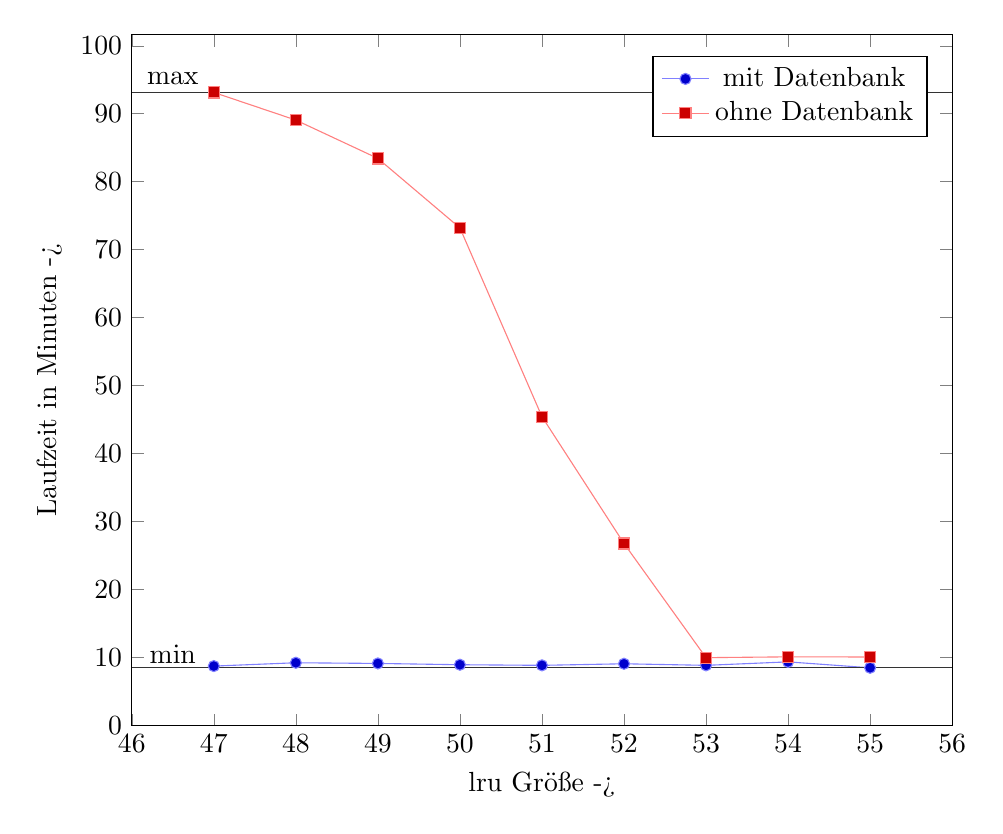
\begin{tikzpicture}
  \begin{axis}[
    width          = 12cm,
    %grid           = both, minor tick num=2,
    %title         = ??,
    xlabel         = \ac{lru} Größe ->,
    ylabel         = Laufzeit in Minuten ->,
    legend pos     = north east,
    ytick distance = 10,
    xmin=46, xmax=56,
    ]

    \tikzstyle{nodetext}=[draw=white, fill=white, draw opacity=0, fill opacity=0, text opacity=1]

    \addplot+[sharp plot, blue!50] coordinates
    {(55, 8.48) (54, 9.35) (53, 8.84) (52, 9.07)
     (51, 8.84) (50, 8.93) (49, 9.12) (48, 9.22) (47, 8.73)};
    \addplot+[sharp plot,  red!50] coordinates
    {(55, 10.07) (54, 10.09) (53, 9.97) (52, 26.77)
     (51, 45.43) (50, 73.20) (49, 83.43) (48, 89.07) (47, 93.14)};

     \addplot[sharp plot,  black!80] coordinates %min
     {(56, 8.48) (46, 8.48)};
     \addplot[sharp plot,  black!80] coordinates %max
     {(56, 93.14) (46, 93.14)};

     \node[nodetext] at (46.5, 10.48) {min};
     \node[nodetext] at (46.5, 95.14) {max};

    \legend{mit Datenbank, ohne Datenbank}
  \end{axis}
\end{tikzpicture}
\caption[Laufzeiten des Systems mit und ohne Datenbank als Cache]{Laufzeiten des Systems (5 Epochs, 53 Datensätze) mit und ohne Datenbank als Cache}\label{cap:analyze}
\end{center}
\end{figure}\label{fig:analyze}
